En la primera secci\'on de este cap\'itulo vimos que, cuando la ecuaci\'on auxiliar de una ecuaci\'on de coeficientes constantes tiene una ra\'iz doble $r$, las funciones $e^{rx}$ y $xe^{rx}$ son soluciones linealmente independientes. En esta secci\'on veremos de d\'onde sale esa segunda soluci\'on y, m\'as importante a\'un, desarrollaremos un m\'etodo que permite encontrar una segunda soluci\'on de \emph{cualquier} ecuaci\'on lineal homog\'enea de segundo orden, siempre que ya conozcamos una. Este m\'etodo se conoce como \textbf{reducci\'on de orden}.

Comencemos con un ejemplo.

\begin{example}
    Sabemos que $y_1=e^{-x}$ es una soluci\'on de
    \[
    y''+2y'+y=0,
    \]
    pues su ecuaci\'on auxiliar es $r^2+2r+1=(r+1)^2=0$. Busquemos una segunda soluci\'on $y_2$ de la forma
    \[
    y_2(x)=u(x)\,e^{-x},
    \]
    donde $u$ es una funci\'on a determinar. Calculamos sus derivadas:
    \[
    y'_2=\left(u'-u\right)e^{-x},\qquad y''_2=\left(u''-2u'+u\right)e^{-x},
    \]
    y reemplazamos en la ecuaci\'on:
    \[
    y_2''+2y_2'+y_2=e^{-x}\Big[\left(u''-2u'+u\right)+2\left(u'-u\right)+u\Big]=e^{-x}u''=0.
    \]
    Todos los t\'erminos con $u$ y $u'$ se cancelan, y nos queda simplemente $u''=0$. Luego $u(x)=C_1x+C_2$, y
    \[
    y_2(x)=\left(C_1x+C_2\right)e^{-x}=C_1\,xe^{-x}+C_2\,e^{-x}.
    \]
    El t\'ermino $C_2e^{-x}$ es un m\'ultiplo de $y_1$, as\'i que no aporta nada nuevo. Tomando $C_1=1$, $C_2=0$ obtenemos la segunda soluci\'on
    \[
    y_2(x)=xe^{-x},
    \]
    que es precisamente la que conoc\'iamos. Como el cociente $y_2/y_1=x$ no es constante, ambas soluciones son L.I.
\end{example}

\begin{figure}[h!]
    \centering
    \begin{subfigure}[b]{0.48\textwidth}
        \centering
        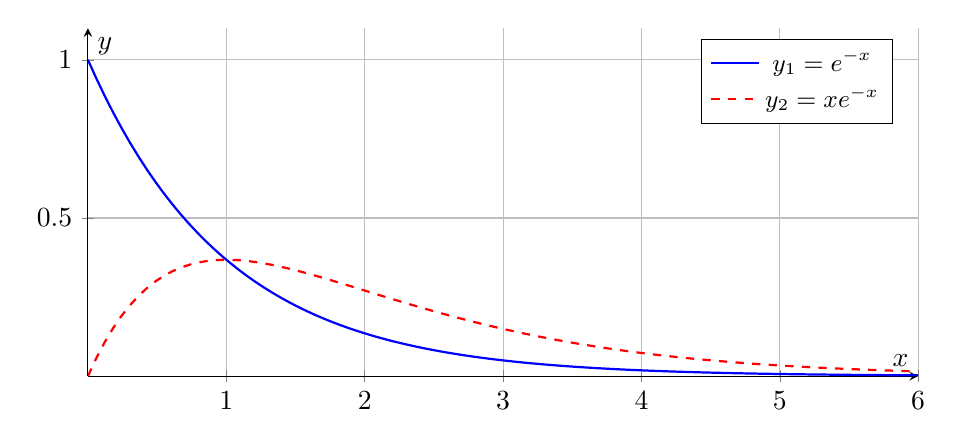
\begin{tikzpicture}
            \begin{axis}[
                axis lines = middle,
                xlabel = $x$, ylabel = {$y$},
                xmin=0, xmax=6, ymin=0, ymax=1.1,
                grid = both,
                width=\textwidth, height=6cm,
                legend pos = north east,
                legend style={font=\small}
            ]
            \addplot[domain=0:6, samples=100, blue, thick] {exp(-x)};
            \addlegendentry{$y_1=e^{-x}$}
            \addplot[domain=0:6, samples=100, red, thick, dashed] {x*exp(-x)};
            \addlegendentry{$y_2=xe^{-x}$}
            \end{axis}
        \end{tikzpicture}
        \caption{Las dos soluciones.}
    \end{subfigure}
    \hfill
    \begin{subfigure}[b]{0.48\textwidth}
        \centering
        \begin{tikzpicture}
            \begin{axis}[
                axis lines = middle,
                xlabel = $x$, ylabel = {$u$},
                xmin=0, xmax=6, ymin=0, ymax=6.5,
                grid = both,
                width=\textwidth, height=6cm,
                legend pos = north west,
                legend style={font=\small}
            ]
            \addplot[domain=0:6, samples=2, violet, thick] {x};
            \addlegendentry{$u=\dfrac{y_2}{y_1}=x$}
            \addplot[domain=0:6, samples=2, gray, dashed] {2};
            \addlegendentry{cociente constante (L.D.)}
            \end{axis}
        \end{tikzpicture}
        \caption{El cociente $u=y_2/y_1$.}
    \end{subfigure}
    \caption{Soluciones de $y''+2y'+y=0$. A la izquierda, $y_2=xe^{-x}$ se obtiene ``modulando'' $y_1=e^{-x}$ con la funci\'on $u(x)=x$. A la derecha, el cociente $u$ no es constante, lo que confirma que las soluciones son L.I.; si lo fuera (l\'inea gris), $y_2$ ser\'ia solo un m\'ultiplo de $y_1$.}
    \label{fig:reduccion_raiz_doble}
\end{figure}

El prop\'osito de esta secci\'on es extender el m\'etodo del ejemplo anterior tanto como sea posible. Para ello, trabajaremos con ecuaciones en \textbf{forma est\'andar}, es decir, con coeficiente $1$ en $y''$:
\[
y''+P(x)y'+Q(x)y=0,
\]
donde $P(x),Q(x)$ son funciones continuas en un intervalo $I$. Si la ecuaci\'on viene dada como $a(x)y''+b(x)y'+c(x)y=0$, basta dividir por $a(x)$ (en un intervalo donde $a(x)\neq0$), de modo que $P=b/a$ y $Q=c/a$.

\subsection*{La f\'ormula de Abel}

Antes de generalizar el m\'etodo, necesitamos un resultado sobre el Wronskiano que ya hemos usado en secciones anteriores y que ahora justificaremos.

\begin{theorem}[F\'ormula de Abel]
    Si $y_1,y_2$ son soluciones de $y''+P(x)y'+Q(x)y=0$ en un intervalo $I$, entonces existe una constante $C$ tal que
    \[
    W[y_1,y_2](x)=C\,e^{-\int P(x)\,dx}\qquad\text{para todo } x\in I.
    \]
    En particular, el Wronskiano de dos soluciones es id\'enticamente cero (si $C=0$) o no se anula en ning\'un punto de $I$ (si $C\neq0$).
\end{theorem}

\begin{proof}
    Derivemos el Wronskiano $W=y_1y_2'-y_1'y_2$:
    \[
    W'=y_1'y_2'+y_1y_2''-y_1''y_2-y_1'y_2'=y_1y_2''-y_1''y_2.
    \]
    Como ambas funciones son soluciones, $y_i''=-Py_i'-Qy_i$ para $i=1,2$. Reemplazando,
    \[
    W'=y_1\left(-Py_2'-Qy_2\right)-\left(-Py_1'-Qy_1\right)y_2=-P\left(y_1y_2'-y_1'y_2\right)=-P\,W.
    \]
    Los t\'erminos con $Q$ se cancelan, y obtenemos la ecuaci\'on lineal de primer orden $W'+PW=0$, cuya soluci\'on es $W=Ce^{-\int P\,dx}$.
\end{proof}

Notemos que la f\'ormula de Abel nos permite conocer el Wronskiano de dos soluciones \emph{sin conocer las soluciones}: solo necesitamos el coeficiente $P(x)$.

\subsection*{El m\'etodo de reducci\'on de orden}

\begin{remark}[Deducci\'on del m\'etodo]
    Supongamos que conocemos una soluci\'on $y_1(x)$ de $y''+Py'+Qy=0$, con $y_1(x)\neq0$ en $I$, y busquemos una segunda soluci\'on de la forma
    \[
    y_2(x)=u(x)\,y_1(x).
    \]
    Derivando,
    \[
    y_2'=u'y_1+uy_1',\qquad y_2''=u''y_1+2u'y_1'+uy_1'',
    \]
    y reemplazando en la ecuaci\'on, agrupamos los t\'erminos con $u$:
    \[
    u\underbrace{\left(y_1''+Py_1'+Qy_1\right)}_{=0}+y_1u''+\left(2y_1'+Py_1\right)u'=0.
    \]
    Como en el ejemplo, los t\'erminos con $u$ desaparecen porque $y_1$ es soluci\'on. Haciendo la sustituci\'on $w=u'$ nos queda
    \[
    y_1w'+\left(2y_1'+Py_1\right)w=0,
    \]
    que es una ecuaci\'on de \emph{primer orden} en $w$: de ah\'i el nombre del m\'etodo. Esta ecuaci\'on es de variables separables:
    \[
    \dfrac{dw}{w}=-\left(\dfrac{2y_1'}{y_1}+P\right)dx\Longrightarrow \ln|w|=-2\ln|y_1|-\int P\,dx+K\Longrightarrow w=\dfrac{C}{y_1^2}\,e^{-\int P\,dx}.
    \]
    Tomando $C=1$ e integrando $u'=w$ (sin constante, pues esta solo agregar\'ia un m\'ultiplo de $y_1$), obtenemos
    \[
    u=\int\dfrac{e^{-\int P(x)\,dx}}{y_1^2(x)}\,dx.
    \]
\end{remark}

Esta f\'ormula tambi\'en se puede obtener directamente de la f\'ormula de Abel. En efecto, si $y_2=uy_1$, entonces
\[
W[y_1,uy_1]=y_1\left(u'y_1+uy_1'\right)-y_1'\,uy_1=y_1^2\,u',
\]
y por la f\'ormula de Abel este Wronskiano debe ser $Ce^{-\int P\,dx}$. Despejando, $u'=\dfrac{Ce^{-\int P\,dx}}{y_1^2}$, que es exactamente lo que obtuvimos. Esto muestra adem\'as que el Wronskiano de $y_1$ e $y_2$ es $e^{-\int P\,dx}\neq0$, por lo que las dos soluciones son siempre L.I.

\begin{theorem}[Reducci\'on de orden]
    Sean $P,Q$ continuas en un intervalo $I$ y sea $y_1$ una soluci\'on de $y''+P(x)y'+Q(x)y=0$ tal que $y_1(x)\neq0$ en $I$. Entonces
    \[
    y_2(x)=y_1(x)\int\dfrac{e^{-\int P(x)\,dx}}{y_1^2(x)}\,dx
    \]
    es una segunda soluci\'on, linealmente independiente con $y_1$, y la soluci\'on general de la ecuaci\'on es $y_h=C_1y_1+C_2y_2$.
\end{theorem}

\begin{remark}[Cuidado con la forma est\'andar]
    La f\'ormula usa el coeficiente $P(x)$ de la ecuaci\'on \emph{en forma est\'andar}. El error m\'as com\'un es aplicarla sin dividir antes por el coeficiente de $y''$, o equivocarse en el signo de $P$. Por ejemplo, en $x^2y''-3xy'+4y=0$ tenemos $P(x)=-\dfrac{3}{x}$, y no $-3x$ ni $\dfrac{3}{x}$.
\end{remark}

El procedimiento completo se resume en el siguiente esquema.

\begin{figure}[h!]
    \centering
    \begin{tikzpicture}[
        paso/.style={draw=bbe, fill=bbe!8, rounded corners=3pt, text width=3.1cm, align=center, minimum height=2.6cm, font=\small, text=black},
        flecha/.style={->, thick, draw=bbe}
    ]
        \node[paso] (a) at (0,0) {\textbf{1.} Escribir en forma est\'andar\\[2pt] $y''+Py'+Qy=0$\\[2pt] e identificar $P$};
        \node[paso] (b) at (3.9,0) {\textbf{2.} Conocer una soluci\'on $y_1$\\[2pt] (dada o por inspecci\'on)};
        \node[paso] (c) at (7.8,0) {\textbf{3.} Por Abel:\\[2pt] $u'=\dfrac{e^{-\int P\,dx}}{y_1^2}$};
        \node[paso] (d) at (11.7,0) {\textbf{4.} Integrar:\\[2pt] $y_2=y_1\displaystyle\int u'\,dx$};
        \draw[flecha] (a) -- (b);
        \draw[flecha] (b) -- (c);
        \draw[flecha] (c) -- (d);
    \end{tikzpicture}
    \caption{Esquema del m\'etodo de reducci\'on de orden.}
    \label{fig:esquema_reduccion}
\end{figure}

Como primera aplicaci\'on, podemos justificar de una vez el caso de la ra\'iz doble.

\begin{example}[El caso de la ra\'iz doble]
    Si $r$ es ra\'iz doble de la ecuaci\'on auxiliar de $ay''+by'+cy=0$, entonces $r=-\dfrac{b}{2a}$, es decir, $2r=-\dfrac{b}{a}$. En forma est\'andar, $P=\dfrac{b}{a}$, y la f\'ormula de reducci\'on de orden con $y_1=e^{rx}$ entrega
    \[
    y_2=e^{rx}\int\dfrac{e^{-\frac{b}{a}x}}{e^{2rx}}\,dx=e^{rx}\int\dfrac{e^{2rx}}{e^{2rx}}\,dx=e^{rx}\int1\,dx=xe^{rx}.
    \]
    Esto explica por qu\'e, en el caso de ra\'iz doble, la segunda soluci\'on es $xe^{rx}$.
\end{example}

\begin{example}
    Se puede verificar que $y_1(x)=x^2$ es una soluci\'on de la ecuaci\'on
    \[
    x^2y''-3xy'+4y=0,\qquad x>0.
    \]
    Para aplicar la f\'ormula, primero dividimos por $x^2$:
    \[
    y''-\dfrac{3}{x}y'+\dfrac{4}{x^2}y=0\Longrightarrow P(x)=-\dfrac{3}{x}.
    \]
    Entonces $-\int P\,dx=\int\dfrac{3}{x}\,dx=3\ln(x)$, luego $e^{-\int P\,dx}=x^3$, y
    \[
    y_2(x)=x^2\int\dfrac{x^3}{x^4}\,dx=x^2\int\dfrac{1}{x}\,dx=x^2\ln(x).
    \]
    Por la f\'ormula de Abel, su Wronskiano es $W[x^2,x^2\ln(x)]=x^3\neq0$ para $x>0$ (puede comprobarlo directamente), as\'i que la soluci\'on general es
    \[
    y_h(x)=C_1x^2+C_2x^2\ln(x).
    \]
\end{example}

\begin{figure}[h!]
    \centering
    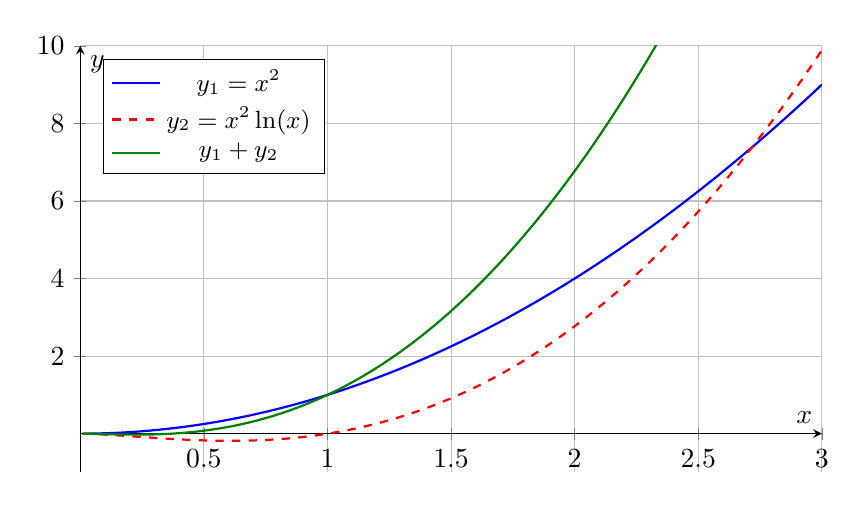
\begin{tikzpicture}
        \begin{axis}[
            axis lines = middle,
            xlabel = $x$, ylabel = {$y$},
            xmin=0, xmax=3, ymin=-1, ymax=10,
            grid = both,
            width = 11cm, height = 7cm,
            legend pos = north west,
            legend style={font=\small}
        ]
        \addplot[domain=0.01:3, samples=150, blue, thick] {x^2};
        \addlegendentry{$y_1=x^2$}
        \addplot[domain=0.01:3, samples=150, red, thick, dashed] {x^2*ln(x)};
        \addlegendentry{$y_2=x^2\ln(x)$}
        \addplot[domain=0.01:3, samples=150, green!50!black, thick] {x^2 + x^2*ln(x)};
        \addlegendentry{$y_1+y_2$}
        \end{axis}
    \end{tikzpicture}
    \caption{Dos soluciones L.I. de $x^2y''-3xy'+4y=0$ y una combinaci\'on de ellas. Notemos que $y_2$ es negativa para $0<x<1$ y cambia de signo en $x=1$, mientras que $y_1$ es siempre positiva: no pueden ser m\'ultiplos una de la otra.}
    \label{fig:reduccion_euler}
\end{figure}

\begin{remark}[\textquestiondown De d\'onde sale $y_1$?]
    El m\'etodo necesita conocer una soluci\'on, y es natural preguntarse c\'omo encontrarla. En algunos casos viene dada en el enunciado o se encuentra por inspecci\'on. Una familia importante son las ecuaciones de \textbf{Cauchy-Euler}, de la forma $ax^2y''+bxy'+cy=0$, donde conviene probar $y=x^r$. Para la ecuaci\'on del ejemplo anterior, reemplazando $y=x^r$ se obtiene
    \[
    r(r-1)-3r+4=r^2-4r+4=(r-2)^2=0,
    \]
    una ra\'iz doble. Tal como en coeficientes constantes la ra\'iz doble produce $e^{rx}$ y $xe^{rx}$, aqu\'i produce $x^2$ y $x^2\ln(x)$.
\end{remark}

\begin{example}
    En la secci\'on de variaci\'on de par\'ametros resolvimos $x^2y''-2xy'+2y=x^3$ usando que $y_1=x$ e $y_2=x^2$ son soluciones de la homog\'enea, y prometimos explicar c\'omo encontrar la segunda. Conociendo solo $y_1=x$, en forma est\'andar tenemos $P(x)=-\dfrac{2}{x}$, luego $e^{-\int P\,dx}=e^{2\ln(x)}=x^2$ y
    \[
    y_2(x)=x\int\dfrac{x^2}{x^2}\,dx=x\int1\,dx=x^2.
    \]
\end{example}

\subsection*{Reducci\'on de orden para ecuaciones no homog\'eneas}

La misma idea funciona para la ecuaci\'on no homog\'enea, y tiene una ventaja notable: a partir de una sola soluci\'on de la homog\'enea, entrega \emph{a la vez} la segunda soluci\'on homog\'enea y una soluci\'on particular.

\begin{remark}[Deducci\'on]
    Busquemos soluciones de $y''+P(x)y'+Q(x)y=F(x)$ de la forma $y=uy_1$, donde $y_1$ es soluci\'on de la homog\'enea. Repitiendo los c\'alculos anteriores, con $w=u'$ llegamos a
    \[
    y_1w'+\left(2y_1'+Py_1\right)w=F,\qquad\text{es decir,}\qquad w'+\left(\dfrac{2y_1'}{y_1}+P\right)w=\dfrac{F}{y_1}.
    \]
    Esta es una ecuaci\'on lineal de primer orden con factor integrante
    \[
    \mu(x)=e^{\int\left(\frac{2y_1'}{y_1}+P\right)dx}=y_1^2(x)\,e^{\int P(x)\,dx}.
    \]
    Multiplicando por $\mu$, la ecuaci\'on queda $(\mu w)'=\dfrac{\mu F}{y_1}$, de donde
    \[
    w=\dfrac{1}{\mu}\left(\int\dfrac{\mu F}{y_1}\,dx+C_2\right),\qquad u=\int w\,dx+C_1.
    \]
\end{remark}

\begin{theorem}[Reducci\'on de orden, caso no homog\'eneo]
    Sean $P,Q,F$ continuas en un intervalo $I$, sea $y_1$ una soluci\'on de la ecuaci\'on homog\'enea $y''+Py'+Qy=0$ con $y_1(x)\neq0$ en $I$, y sea $\mu(x)=y_1^2(x)\,e^{\int P(x)\,dx}$. Entonces la soluci\'on general de
    \[
    y''+P(x)y'+Q(x)y=F(x)
    \]
    es $y=C_1y_1+C_2y_2+y_p$, donde
    \[
    y_2(x)=y_1(x)\int\dfrac{dx}{\mu(x)},\qquad y_p(x)=y_1(x)\int\dfrac{1}{\mu(s)}\left(\int^{s}\dfrac{\mu(t)F(t)}{y_1(t)}\,dt\right)ds.
    \]
\end{theorem}

Notemos que $\dfrac{1}{\mu}=\dfrac{e^{-\int P\,dx}}{y_1^2}$, de modo que la $y_2$ de este teorema es la misma que obtuvimos en el caso homog\'eneo.

\begin{remark}[Dos caminos]
    Si conocemos una soluci\'on $y_1$ de la homog\'enea, para resolver la ecuaci\'on no homog\'enea tenemos dos opciones:
    \begin{enumerate}[label=\roman*)]
        \item aplicar directamente el teorema anterior, que entrega $y_2$ e $y_p$ al mismo tiempo, o
        \item usar reducci\'on de orden solo para encontrar $y_2$, y luego variaci\'on de par\'ametros para encontrar $y_p$.
    \end{enumerate}
    Ambos caminos conducen a la misma soluci\'on general; conviene elegir el que produzca integrales m\'as sencillas.
\end{remark}

\begin{example}
    Resuelva la ecuaci\'on diferencial
    \[
    x^2y''+3xy'+y=4\ln(x),\qquad x>0,
    \]
    sabiendo que $y_1(x)=x^{-1}$ es una soluci\'on de la ecuaci\'on homog\'enea asociada.

    Antes de comenzar, llevamos la ecuaci\'on a su forma est\'andar dividiendo por $x^2$:
    \[
    y''+\dfrac{3}{x}y'+\dfrac{1}{x^2}y=\dfrac{4\ln(x)}{x^2},
    \]
    e identificamos
    \[
    P(x)=\dfrac{3}{x},\qquad F(x)=\dfrac{4\ln(x)}{x^2},\qquad y_1(x)=x^{-1}.
    \]
    Calculamos el factor integrante:
    \[
    e^{\int P\,dx}=e^{3\ln(x)}=x^3,\qquad \mu(x)=y_1^2\,e^{\int P\,dx}=x^{-2}\cdot x^3=x.
    \]
    Resolvemos primero la integral interior:
    \[
    \int\dfrac{\mu F}{y_1}\,dx=\int x\cdot\dfrac{4\ln(x)}{x^2}\cdot x\,dx=\int4\ln(x)\,dx=4x\ln(x)-4x,
    \]
    donde integramos por partes. Luego,
    \[
    w=\dfrac{1}{\mu}\left(4x\ln(x)-4x+C_2\right)=4\ln(x)-4+\dfrac{C_2}{x},
    \]
    e integrando nuevamente,
    \[
    u=\int\left(4\ln(x)-4+\dfrac{C_2}{x}\right)dx=4x\ln(x)-8x+C_2\ln(x)+C_1.
    \]
    Finalmente, la soluci\'on general es $y=u\,y_1$:
    \[
    y(x)=x^{-1}\left(4x\ln(x)-8x+C_2\ln(x)+C_1\right)=\underbrace{C_1x^{-1}}_{C_1y_1}+\underbrace{C_2\,x^{-1}\ln(x)}_{C_2y_2}+\underbrace{4\ln(x)-8}_{y_p}.
    \]
    Notemos que, a partir de la sola soluci\'on $y_1=x^{-1}$, obtuvimos la segunda soluci\'on homog\'enea $y_2=x^{-1}\ln(x)$ y la soluci\'on particular $y_p=4\ln(x)-8$. Como en el ejemplo anterior, esta es una ecuaci\'on de Cauchy-Euler: probando $y=x^r$ en la homog\'enea se obtiene $(r+1)^2=0$, una ra\'iz doble, lo que explica la aparici\'on de $\ln(x)$ en $y_2$.
\end{example}

\begin{figure}[h!]
    \centering
    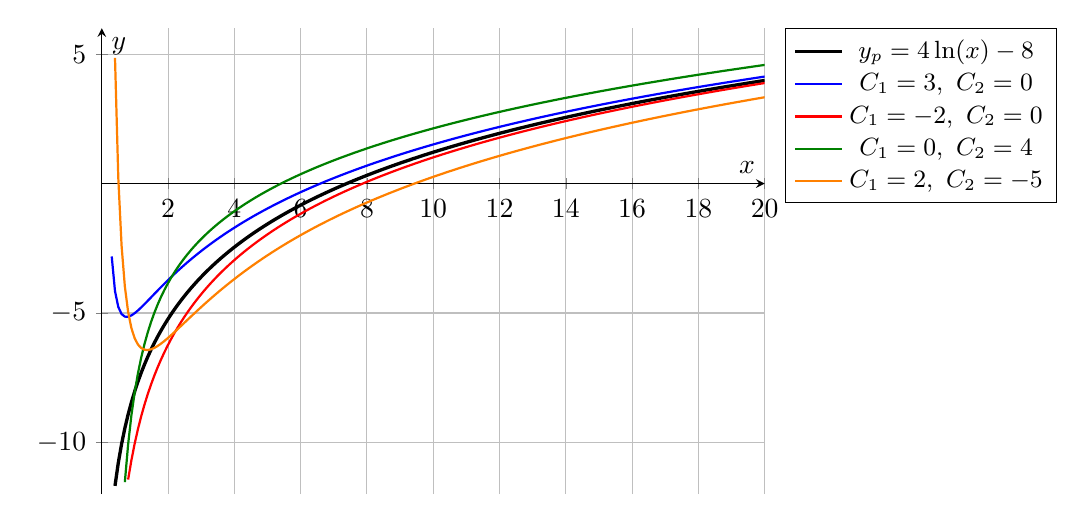
\begin{tikzpicture}
        \begin{axis}[
            axis lines = middle,
            xlabel = $x$, ylabel = {$y$},
            xmin=0, xmax=20, ymin=-12, ymax=6,
            restrict y to domain=-12:6,
            grid = both,
            width = 10cm, height = 7.5cm,
            legend pos = outer north east,
            legend style={font=\small}
        ]
        \addplot[domain=0.3:20, samples=200, black, very thick] {4*ln(x) - 8};
        \addlegendentry{$y_p=4\ln(x)-8$}
        \addplot[domain=0.3:20, samples=200, blue, thick] {4*ln(x) - 8 + 3/x};
        \addlegendentry{$C_1=3,\ C_2=0$}
        \addplot[domain=0.3:20, samples=200, red, thick] {4*ln(x) - 8 - 2/x};
        \addlegendentry{$C_1=-2,\ C_2=0$}
        \addplot[domain=0.3:20, samples=200, green!50!black, thick] {4*ln(x) - 8 + 4*ln(x)/x};
        \addlegendentry{$C_1=0,\ C_2=4$}
        \addplot[domain=0.3:20, samples=200, orange, thick] {4*ln(x) - 8 + 2/x - 5*ln(x)/x};
        \addlegendentry{$C_1=2,\ C_2=-5$}
        \end{axis}
    \end{tikzpicture}
    \caption{Algunas soluciones de $x^2y''+3xy'+y=4\ln(x)$. Como $y_1=x^{-1}$ e $y_2=x^{-1}\ln(x)$ tienden a cero cuando $x\to\infty$, todas las soluciones se acercan a la soluci\'on particular $y_p=4\ln(x)-8$ (negro): la parte homog\'enea es un ``transiente'' que se desvanece.}
    \label{fig:reduccion_no_homogenea}
\end{figure}
